\section{mbeddr Debugger Framework}
\label{mbeddrDebugger}
\label{mbeddrDebuggerFramework}



mbeddr comes with a debugger, which allows users to debug their mbeddr code 
on the abstraction levels of the used languages. 
For that, each language contributes a debugger extension, which is
built with a framework also provided by mbeddr~\cite{DBLP:conf/adaEurope/AdaEuropeDeb}.
Those extensions are always language-specific in contrast to 
domain-specific debuggers (\eg the moldable
debugger~\cite{DBLP:conf/sle/ChisGN14}), 
which provide application-specific debug actions and views on the program
state.
Hence, debugging support is implemented specifically for the language
by lifting the call stack/program state from the base-level to the
extension-level (see \fig{infoFlow}) and stepping/breakpoints
vice versa. 

\begin{figure}[h]
  \vspace{-3mm}
  \centering
    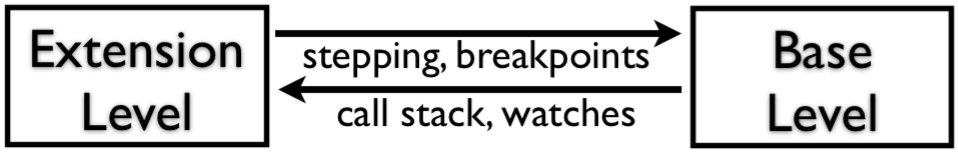
\includegraphics[width=5.5cm]{./figures/two-levels.png} 
    \vspace{-2mm}
    \caption{Flow of debug information between base and
    extension level~\cite{DBLP:conf/adaEurope/AdaEuropeDeb}}
  \label{infoFlow}
  \vspace{-2mm}
\end{figure}



The debugger framework can be separated into two different parts: First, a
\ac{DSL} and a set of interfaces (shown in \fig{specabs}) for specifying the
debugging semantics of language concepts. 
Second, a runtime for executing those specifications and
thus achieving the mapping described in~\fig{infoFlow}. 

In this section, we provide an overview of the specification part (see
\fig{specabs}) that is required for understanding how the debugger extension
for \emph{MUnit} is built.
While this paper concentrates on testing debuggers for extensible languages,
we have published another paper~\cite{DBLP:conf/adaEurope/AdaEuropeDeb}
describing details about the debugger framework and its implementation
with \ac{MPS}.


\subsection{Breakpoints}
\ic{Breakable}s are concepts (\eg \ic{Statement}s) on which
we can set breakpoints to suspend the program execution.


\subsection{Watches}

\ic{WatchProvider}s are translated to low-level watches (\eg
\ic{Argument}) or represent watches on the extension-level.
They are declared inside \ic{WatchProviderScope}s (\eg
\ic{StatementList}), which is a nestable context.

\subsection{Stepping} 
\ic{Steppable}s define where program execution must suspend
next, after the user \emph{steps over} 
an instance of \ic{Steppable} (\eg \ic{Statement}). If a
\ic{Steppable} contains a \ic{StepIntoable} (\eg \ic{FunctionCall}), 
then the \ic{Steppable} also supports \emph{step into}. \ic{StepIntoable}s are
concepts that branch execution into a \ic{SteppableComposite} (\eg \ic{Function}).

All stepping is implemented by setting low-level breakpoints and then resuming
execution until one of these breakpoints is hit (approach is based
on~\cite{Wu06grammar}). The particular stepping behavior is realized through 
stepping-related concepts by utilizing \ic{DebugStrategies}.

\subsection{Call Stack}
\ic{StackFrameContributor}s are
concepts that have callable semantics on the extension-level or are
translated to low-level callables (\eg \ic{Function}s). While the latter do
not contribute any \ic{StackFrame}s to the high level call stack, the former
contribute at least one \ic{StackFrame}.

\begin{figure}[h]
  \vspace{-2mm}
  \centering
    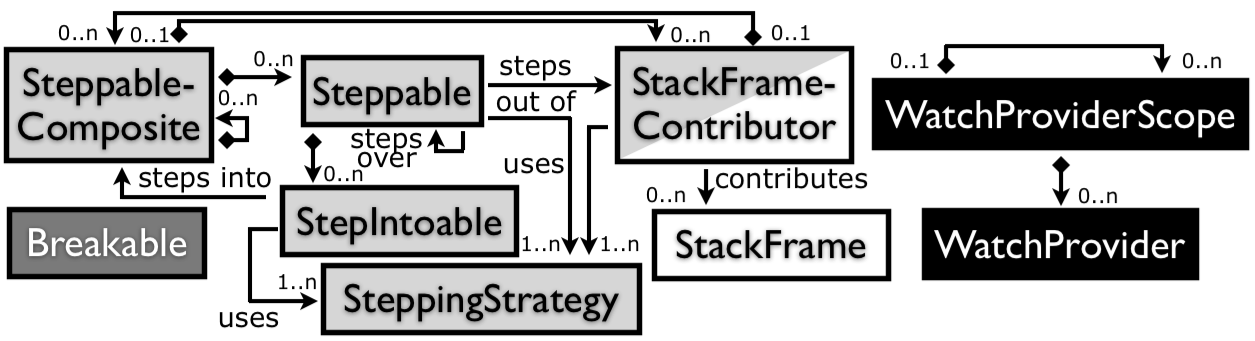
\includegraphics[width=8.75cm]{./figures/debugger-concepts.png} 
    \vspace{-4mm}
    \caption{Meta-model used for specifying the debugging semantics of language
    concepts~\cite{DBLP:conf/adaEurope/AdaEuropeDeb}. Colors indicate the
    different debugging aspects} 
  \label{specabs}
  \vspace{-2mm}
\end{figure}

\section{Debugger Extension for the MUnit Language}

This section describes the implementation of a debugger extension
for the \emph{MUnit} language. This extension is defined with the mbeddr
debugger specification \ac{DSL} and the abstractions of the debugging
meta-model shown in \fig{specabs}.

\subsection{Breakpoints}  To enable
breakpoints on \ic{AssertStatement}s, 
an implementation of the \ic{Breakable} interface is required.
\ic{Assert- Statement} is derived from \ic{Statement} that already implements
this interface, thus breakpoints are already supported.

\subsection{Watches} 

Since \ic{ExecuteTestExpression}'s  stack frame is not shown in the high-level
call stack, none of its watches are mapped.
In contrast,  stack frames for \ic{Testcase}s are visible thus we need
to consider its watches. In case of \ic{Testcase}, the 
\ic{LocalVariableDeclaration} \_f has no corresponding
representation on the extension-level, and should therefore not be shown. The
mbeddr debugger framework has a pessimistic approach for lifting watches:
watches that should not be shown in the \ic{UI} are marked as \emph{hidden}.
Otherwise, the debugger shows the low-level watch (in this case the C local
variable \_f) with its respective value.

\begin{lstlisting}[frame=single,language=debuggerDSL]
hide local variable with identifier "_f";
\end{lstlisting}

\subsection{Stepping} 

\ic{AssertStatement} is a \ic{Statement}, which
already provides \emph{step over} behavior. However, to be able to 
\emph{step into} the \emph{condition} we overwrite \ic{Statement}'s 
\emph{step into} behavior: 
\begin{lstlisting}[language=debuggerDSL,frame=single]
break on nodes to step-into: this.expr;
\end{lstlisting}

\ic{break on nodes} searches in \emph{condition}
for instances of \ic{StepIntoable} and contributes their 
\emph{step into} strategies.

\ic{ExecuteTestExpression} implements \ic{StepIntoable} to allow 
\emph{step into} the referenced \ic{Testcase}s. A  
minimal implementation puts a breakpoint in each \ic{Testcase}:
\begin{lstlisting}[language=debuggerDSL,frame=single]
foreach testRef in this.tests { 
   break on node: testRef.test.body.statements.first;
}
\end{lstlisting}

\subsection{Call Stack}
\label{CallStackDebuggerDef}

\ic{Testcase} and \ic{ExecuteTestExpression} are translated to 
base-level callables and therefore implement
\ic{StackFrame- Contributor}. They contribute \ic{StackFrame}s, 
each is linked to a base-level stack frame and
states whether it is visible in the extension-level call stack or not.

The implementation of  \ic{ExecuteTestExpression} links the
low-level stack frame to the respective instance (see listing below).
Further, it hides the frame from the high-level call stack, since
\ic{ExecuteTestExpression} has no callable semantics.

\begin{lstlisting}[language=debuggerDSL,frame=single]
contribute frame mapping for frames.select(name=getName());
\end{lstlisting}

Similarly the mapping for \ic{Testcase} also requires linking the
low-level stack frame to the respective instance. However, 
it declares to \emph{show} the stack frame in the high-level call stack:
\begin{lstlisting}[language=debuggerDSL,frame=single]
String frameName = "test_" + this.name;
contribute frame mapping for frames.select(name=frameName);
\end{lstlisting}
Further, we provide the name of the actual \ic{Testcase}, which is represented
in the call stack view: Consider \lst{lst:generatedUT}, where we would
show the name \ic{forTest} instead of \ic{test\_forTest}.